\documentclass{patmorin}
\usepackage{graphicx}
\usepackage{pat}

\setlength{\parskip}{1ex}
\title{\MakeUppercase{How to Thue-Colour a 3-Branched Tree}}

\author{Bellairs 2016 Pre-Group}

\begin{document}
\maketitle 

\section{Thue-Colouring $T^3_n$}

Let $T^3_n$ be a tree having a root $r$ of degree 3 and the three subtrees of $r$ are each paths of length $n$.  We will prove that $T^3_n$ has a nonrepetitivie 3-colouring.  Our proof uses the Prouhet-Thue-Morse sequence and some of its properties, which we review here.

For each $i\in N$, define $s_i$ as the parity of the binary representation
of $i$.  The sequence $s=s_0,s_1,\ldots$ is known as the Prouhet-Thue-Morse
sequence.  Alternatively, we can say that $s_0=0$ and, for every $i\ge 1$,
$s_{2^{i}},\ldots,s_{2^{i+1}-1}=\overline{s_0,\ldots,s_{2^{i}-1}}$.
The first few bits of this sequence are:
\[
   01\:\: 10\:\: 1001\:\: 10010110\:\: 1001011001101001\ldots
\]
The Prouhet-Thue-Morse string has the important property of being
\emph{overlap free}: It does not contain any block of the form $awawa$,
where $a\in\{0,1\}$ and $w\in\{0,1\}^*$.

Using $s$, one can form an infinite sequence, $r$, over $\{0,1,2\}$
by taking the gaps between successive 0's:
\[
   s = 0\underbrace{11}_20\underbrace{1}_10\underbrace{}_00\underbrace{11}_{2}0\underbrace{0}_0\underbrace{1}_10\underbrace{11}_20\ldots
\]

\[
    r=2,1,0,2,0,1,2,1,0,1,2,0,2,1,0,2,0,1,2,0,2,1,0,1,\ldots
\]
The overlap-freeness of $s$, in particular, the lack of any block of the
form $0w0w0$ ensures that $r$ is nonrepetitive. Another useful property
of $r$ is that, if it contains some block $b$ then it contains infinitely
many occurrences of $b$.  

Note that the overlap-freeness of $s$ also implies that $r$ does not
contain the block $2,1,2$ since this would mean that $s$ contains
the block
\[ 
   01\underbrace{10101}_\text{overlap}10 \enspace .
\]

\begin{thm}
  $T^3_n$ has a nonrepetitive 3-colouring
\end{thm}

\begin{proof}
Let $t=20\:212010212\:021$.  Notice that $t$ is nonrepetitive.
Furthermore, if $r_{i,\ldots,i+4}=12021$, then $t,r_{i+5},r_{i+6},\ldots$
is also nonrepetitive.  Finally, if $r_{i,\ldots,i+3}=1202$, then
$\overleftarrow{t},r_{i+4},r_{i+5},\ldots,$ is also nonrepetitive.
Finally, we note that the block $12021$ (and hence also $1202$) appears
in $r$ so infinitely many such values of $i$ exist.  In particular,
there is an $i > n+20$ such that $r_{i,\ldots,i+4}=12021$. Therefore,
the following colouring of $T^3_n$ works:
\begin{center}
  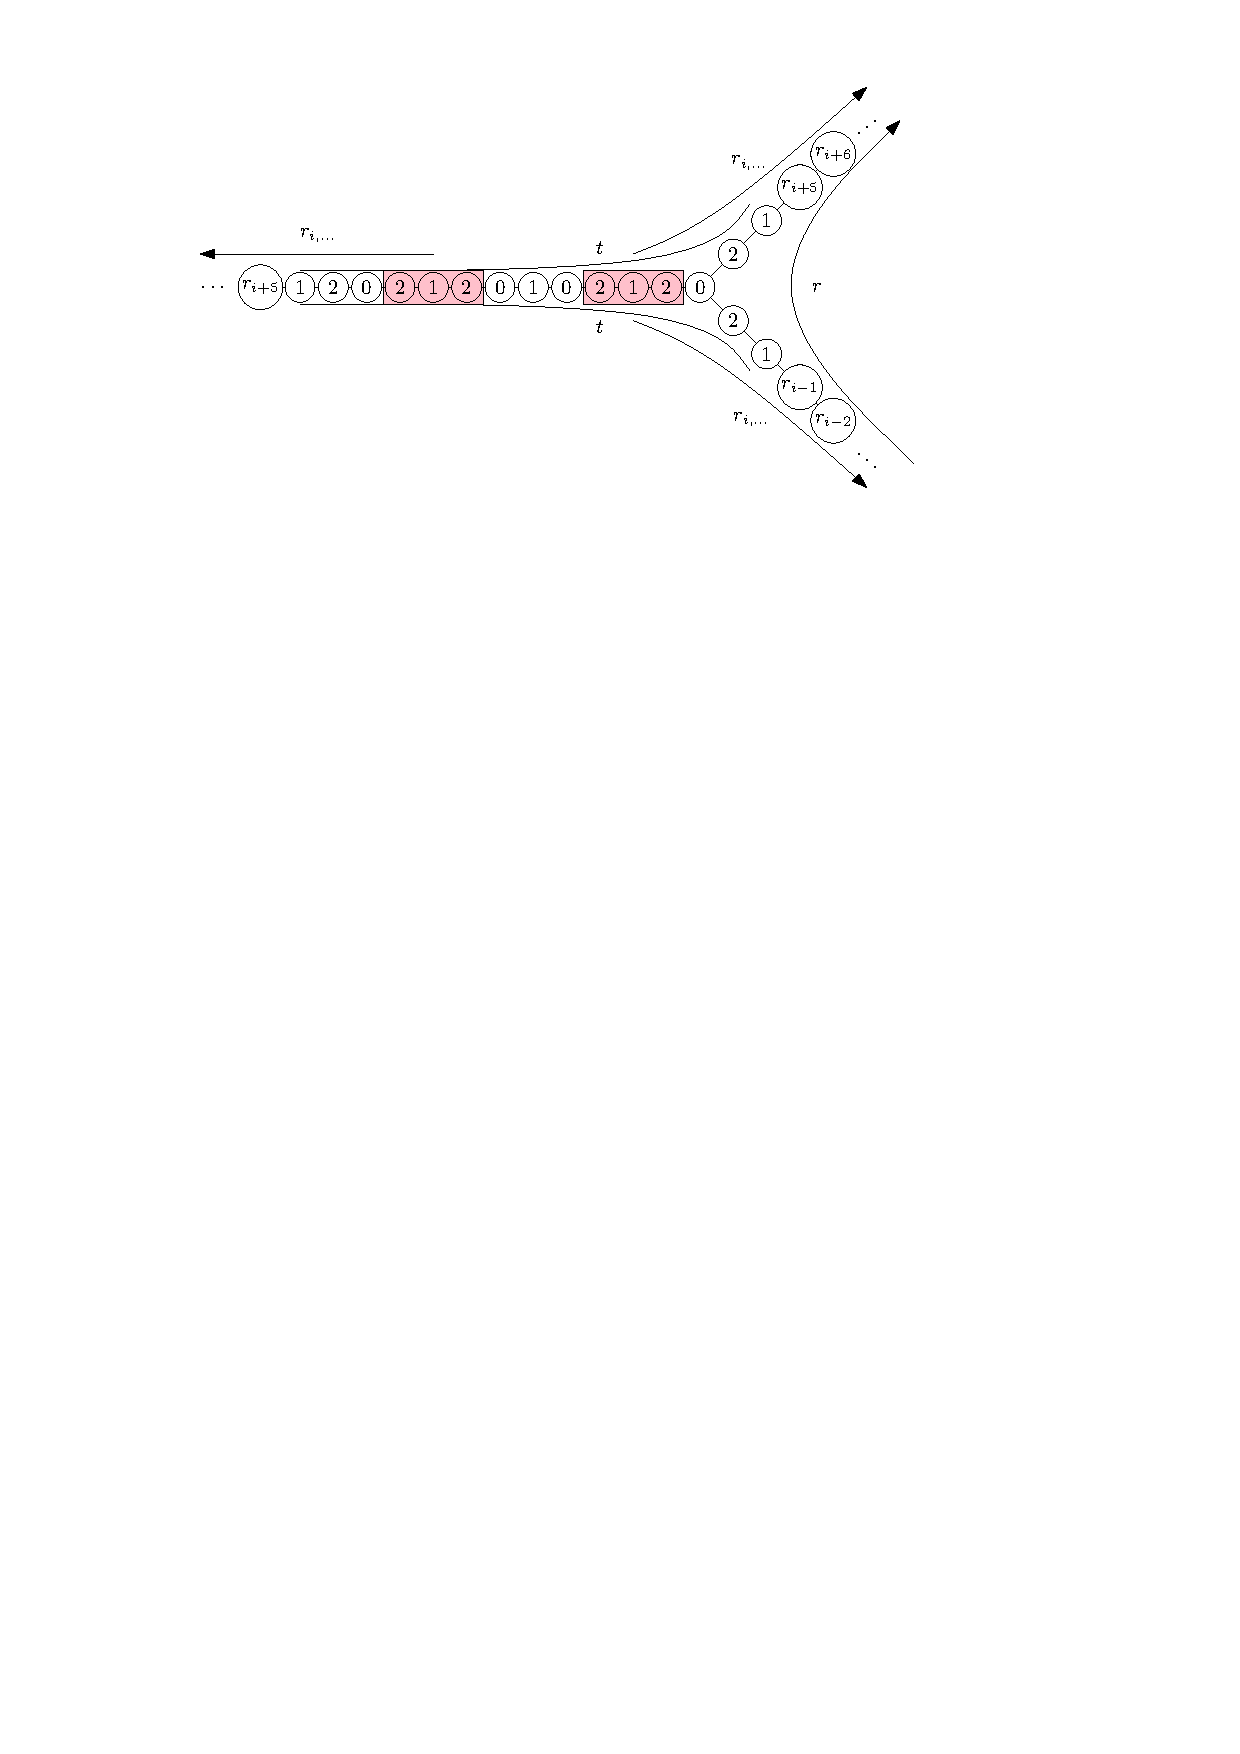
\includegraphics{t3n}
\end{center}
Why does this work?  Referring to the figure above, any path contained
in the two right branches is coloured with a substring of $r$, so it is
coloured nonrepetitively.  Therefore, if there is a path that forms a
repetition, it must use some of the left branch.  The path must use some
part of the left branch other than the trailing $120$ since otherwise the
colour sequence we obtain also appears in $r$.  For the same reason, the
path must use some part of the left branch to the right of $12021$.

Therefore, any repetitively coloured path must include the colour sequence $212$ that appears in $t$.  Some straightforward verification (that we have to do anyway to ensure that $t$ is nonrepetitive) then shows that the path must include both occurrence of $212$ in $t$.  Since the block $212$ does not appear anywhere else in $r$, there must be one occurrence of $212$ in each of the first and second halfs of the path, which leaves only these possibilities:
\[
   \begin{array}{cccccc|cccccc}
       1 & 2 & 0 & 2 & 1 & 2 & 0 & 1 & 0 & 2 & 1 & 2 \\
       2 & 0 & 2 & 1 & 2 & 0 & 1 & 0 & 2 & 1 & 2 & 0 \\
       0 & 2 & 1 & 2 & 0 & 1 & 0 & 2 & 1 & 2 & 0 & 2 \\
       2 & 1 & 2 & 0 & 1 & 0 & 2 & 1 & 2 & 0 & 2 & 1 \\
   \end{array} \enspace,
\]
none of which is a repetition.
\end{proof}

\section{Remarks}

Unfortunately, because the sequence $t$ is so long, this proof doesn't
look like it will generalize to arbitray trees.  If we continue with
the current line of argument, we may be able to prove that any (binary)
tree that has had all its edges subdivided $k$ times can be (facially)
nonrepetitively 3-coloured.

\end{document}
